\documentclass[12pt, a4paper, twoside]{pancake-book}

% NOTE *** preamble ***
\setlength{\headheight}{14.49998pt} % make latex stop complaining!

% simpler commands
\renewcommand*{\bf}[1]{\textbf{#1}}
\renewcommand*{\it}[1]{\textit{#1}}
\renewcommand*{\tt}[1]{\texttt{#1}}

% math macros
\newcommand*{\f}[2]{\frac{#1}{#2}}
\newcommand*{\slf}[2]{\slashfrac[auto]{#1}{#2}}
\newcommand*{\R}{\mathbb{R}}
\newcommand*{\Z}{\mathbb{Z}}
\newcommand*{\Q}{\mathbb{Q}}
\newcommand*{\N}{\mathbb{N}}

% define colours used throughout the document
\definecolor{accent}{HTML}{EF476F}
\definecolor{razz}{HTML}{DB3069} % pink -- all of these colours are very vibrant
\definecolor{cobalt}{HTML}{1446A0} % blue
\definecolor{naples}{HTML}{F5D547} % yellow

% wrap figures
\usepackage{wrapfig}

% essentials for math + chemistry
\usepackage{mathtools, amsthm, amssymb, amsmath}
\usepackage{derivative}
\usepackage{physics2}
\usephysicsmodule[tightbraces=true]{ab}
\usepackage{chemformula, chemmacros}
\usepackage{cancel}

\usepackage{siunitx}
\sisetup{
	mode=match,
	propagate-math-font=true,
	reset-math-version=false,
	reset-text-family=false,
	reset-text-series=false,
	reset-text-shape=false,
	text-family-to-math=true,
	text-series-to-math=true,
}
\DeclareSIUnit{\conc}{\mol\per\deci\meter\cubed}
\DeclareSIUnit{\concrate}{\conc\per\second}
\DeclareSIUnit{\year}{year}
\DeclareSIUnit{\electron}{electron}
\DeclareSIUnit{\atom}{atom}
\DeclareSIUnit{\epera}{\electron\per\atom}
\DeclareSIUnit{\atm}{atm}

% fonts
\usepackage[scaled]{FiraSans} % for the sans font
\usepackage{newpx}
\usepackage[scaled]{FiraMono}

\title{SJChO: Homework}
\author{Darren \color{accent} Yap}
\date{2024}

\usepackage{pgfplots, pgfplotstable}
\pgfplotstableset{col sep=comma}
\usetikzlibrary{%
	positioning,% Relative positioning etc.
	calc,% Calculate distances, coordinates etc.
	shapes, % For cross ou t
	backgrounds,% Draw on background layer
	fit,% Fit new node around existing coordinates
	decorations,
	arrows,
	arrows.spaced,
	intersections,
	% trees,
	% circuits.ee.IEC,% Electrical engineering circuits lib
	patterns,
	3d,
	tikzmark,% Marks/coordinates at arbitrary positions
}%
\usepgfplotslibrary{%
	colorbrewer,
	units,
	dateplot,
	fillbetween,
	groupplots,
}%
\pgfplotscreateplotcyclelist{mod RdYlBu3}{
	{accent},
	{cobalt},
	{naples},
	% {black!50},
}
\pgfplotscreateplotcyclelist{mod mark list}{% Modify predefined to start without mark
	every mark/.append style={solid,fill=\pgfplotsmarklistfill}\\
	every mark/.append style={solid,fill=\pgfplotsmarklistfill},mark=*\\
	every mark/.append style={solid,fill=\pgfplotsmarklistfill},mark=square*\\
	every mark/.append style={solid,fill=\pgfplotsmarklistfill},mark=triangle*\\
	every mark/.append style={solid},mark=star\\
	every mark/.append style={solid,fill=\pgfplotsmarklistfill},mark=diamond*\\
	every mark/.append style={solid,fill=\pgfplotsmarklistfill!40},mark=otimes*\\
	every mark/.append style={solid},mark=|\\
	every mark/.append style={solid,fill=\pgfplotsmarklistfill},mark=pentagon*\\
}%
\pgfplotsset{
	width=8cm,
	compat=1.16,
	clip mode=individual,
	label style={font=\small},
	tick label style={%
		font=\small,%
		/pgf/number format/1000 sep={\,}% Small space instead of comma
		/pgf/number format/precision=3,
		/pgf/number format/fixed,
		/pgf/number format/fixed zerofill,
	},
	legend style={%
		at={(0.5, 1.05)},
		anchor=south,
		legend columns=-1,
		font=\footnotesize,%
		draw=none,
		fill=none,
	},%
	colormap/viridis,
	unit code/.code 2 args={\unit{#1#2}},
	unit markings={slash space},
	every axis plot post/.append style={
		align=center,
		ultra thick,
		axis lines=left,
		axis x line=bottom,
		axis y line=left,
		axis line style={semithick},
		enlargelimits=0.05,
	},%
	cycle multi list={%
		mod mark list\nextlist% Just in case; likely never reached
		linestyles*\nextlist
		%% Iterate through last one first; if at end, start anew using
		%% next in parent (linestyles *):
		mod RdYlBu3%
	},%
}

\usepackage{tcolorbox}
\tcbuselibrary{breakable, skins}
\newtcbox{\hil}[1][accent]{
	on line,
	arc=0pt,
	outer arc=0pt,
	colback=#1!25!white,colframe=#1,
	boxsep=0pt,left=1pt,right=1pt,top=2pt,bottom=2pt,
	boxrule=0pt,bottomrule=1pt,toprule=1pt,
	breakable,enhanced jigsaw,
	before=\noindent\begingroup,after=\endgroup,
}

\usepackage{hyperref, bookmark}
\hypersetup{
	hidelinks,
	colorlinks=true,
	breaklinks=true,
	urlcolor=razz,
	bookmarksopen=false,
	pdftitle={SJChO},
	pdfauthor={Darren Yap},
	linkcolor=cobalt,
}

\begin{document}
\maketitle
\tableofcontents

% \setcounter{part}{5}
\setcounter{chapter}{5}


% *** Kinetics ***
\chapter{Reaction Kinetics}
\section{Homework: Reaction Kinetics}
\subsection{Redox}
\subsubsection{Problem}
Hydrogen peroxide reacts with acidified iodide ions, liberating iodine.
In investigations of this reaction, the following results were
obtained (Table~\ref{tab:h2o2}).
\begin{table}[htpb]
	\centering
	\footnotesize
	\begin{tabular}{l r r r r}
		\toprule
		Experiment & \ch{[H2O2]}/\unit{\milli\conc} & \ch{[I^-]}/\unit{\milli\conc} & \ch{[H^{+}]}/\unit{\milli\conc} & Initial rate/\unit{\milli\concrate} \\
		\midrule
		1          & \num{10.0}                     & \num{9.0}                     & \num{10.0}                      & \num{2.30e-3}                       \\
		2          & \num{34.0}                     & \num{9.0}                     & \num{10.0}                      & \num{7.82e-3}                       \\
		3          & \num{34.0}                     & \num{13.5}                    & \num{10.0}                      & \num{1.75e-2}                       \\
		4          & \num{34.0}                     & \num{9.0}                     & \num{24.0}                      & \num{7.82e-3}                       \\
		\bottomrule
	\end{tabular}
	\caption{Results for reaction between \ch{H2O2} and \ch{I-}}
	\label{tab:h2o2}
\end{table}

\begin{enumerate}
	\item Determine the rate equation of this reaction.
	\item Calculate the rate constant and state its units.
\end{enumerate}

\subsubsection{Solution}
Since the initial rate increases linearly with \ch{[H2O2]}, the reaction
is first-order w.r.t. \ch{[H2O2]}. The reaction is second-order w.r.t. \ch{[I^-]}
and zeroth-order w.r.t. \ch{[H^{+}]}. Therefore, the rate equation is (Equation~\ref{eq:rateeq-h2o2})

\begin{equation}
	\color{accent}
	v = k \ch{[H2O2]} {\ch{[I^-]}}^2
	\label{eq:rateeq-h2o2}
\end{equation}

We can substitute the values from Experiment 1 into Equation~\ref{eq:rateeq-h2o2}.
\begin{align*}
	\num{2.30e-3} & = k \left(10.0\right) \ab(9.0)^2                         \\
	k             & = \f{\num{2.30e-3}}{\num{810.0}}                         \\
	              & = \color{accent} \qty{2.84e-6}{mmol^{-2}.dm^{-6}.s^{-1}} \\
\end{align*}

\subsection{Decomposition Graphs}
\subsubsection{Problem}
The decomposition of \ch{N2O4} is found to be \textbf{first-order}
with respect to \ch{[N2O4]} (Figure~\ref{fig:graphs}).
Which of the following graphs confirms the above finding? For the graphs that are incorrect, copy the axes
and sketch the correct shape of the graph.
\begin{figure}
	\centering
	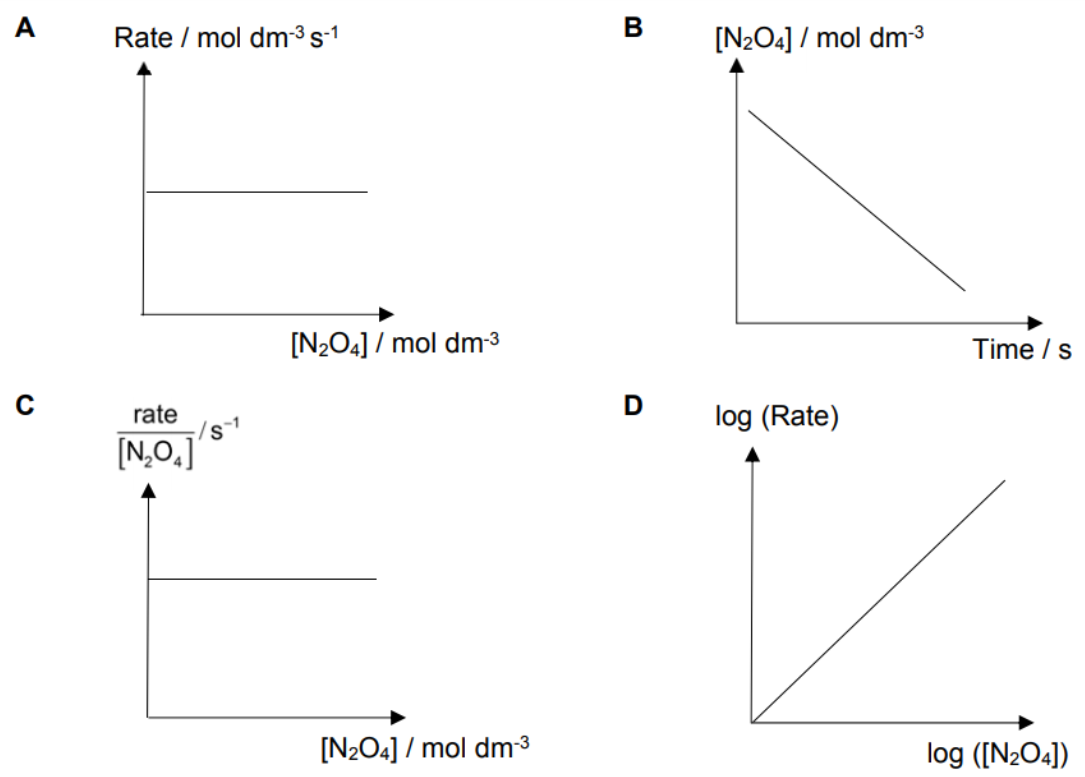
\includegraphics[width=0.90\linewidth]{assets/06_n2o4.png}
	\caption{Various graphs of the decomposition of \ch{N2O4}}
	\label{fig:graphs}
\end{figure}

\begin{itemize}
	\item Graph \textbf{A} is {\color{accent} incorrect}. It illustrates a zeroth-order decomposition instead of a first-order one. The correct shape is:
	      \begin{center}
		      \begin{tikzpicture}
			      \begin{axis}[
					      ticks=none,
					      xmin=0,ymin=0,xmax=3,ymax=3,
					      xlabel={\(\slf{\ch{[N2O4]}}{\unit{\conc}}\)},
					      ylabel={\(\slf{v}{\unit{\concrate}}\)},
				      ]
				      \addplot+[dotted]{1.5};
				      \addplot{x};
			      \end{axis}
		      \end{tikzpicture}
	      \end{center}
	\item Graph \textbf{B} is {\color{accent} correct}. Since \(v = -\odv{\ch{[N2O4]}}/{t}\)
	      and \ch{N2O4} undergoes first-order decomposition, \ch{[N2O4]} should decrease
	      linearly too.
	\item Graph \textbf{C} is {\color{accent} correct}. Since \(v = k\ch{[N2O4]}\),
	      \(k = \slf{v}{\ch{[N2O4]}}\), a constant.
	\item Graph \textbf{D} is {\color{accent} incorrect}. The graph of \(v\) against
	      \ch{[N2O4]} is linear, so the graph of \(\log v\) against \(\log \ch{[N2O4]}\)
	      should follow a logarithmic curve:
	      \begin{center}
		      \begin{tikzpicture}
			      \begin{axis}[
					      ticks=none,
					      xmin=0,ymin=-1,xmax=5,ymax=5,
					      xlabel={\(\log \ch{[N2O4]}\)},
					      ylabel={\(\log v\)},
					      ticks=none,
				      ]
				      \addplot+[dotted]{x};
				      \addplot{ln x};
			      \end{axis}
		      \end{tikzpicture}
	      \end{center}
\end{itemize}

\subsection{Carbon Dating}
\subsubsection{Problem}
Carbon-14 dating is a technique used to estimate the age of organic material. A living organism constantly exchanges carbon with the environment, thus the amount
of radioactive carbon-14 in the organism stays constant at around 1 part per trillion.
When the organism dies, the amount of carbon-14 starts to decrease due to radioactive decay, following first-order kinetics with a decay constant of \qty{1.21e-4}{\per\year}.

\begin{enumerate}
	\item The human body comprises roughly \qty{16}{\kilo\gram} of carbon. Estimate the number of carbon-14 atoms present in a living human.
	\item When one carbon-14 atom decays, one electron is emitted. Calculate the rate of emission of electrons from a living human, giving your answer in electrons per second.
	\item The rate of electron emission from an ancient Egyptian mummy was detected to be \qty{2000}{electron.s^{-1}}. Estimate the age of the mummy.
\end{enumerate}

\begin{align*}
	\text{Total mass of all \ch{^{14}C} atoms} & = \qty{16e-12}{\kilogram}                            \\
	                                           & = \qty{1.6e-11}{\kilogram}                           \\
	                                           & = \qty{1.6e-8}{\gram}                                \\
	\\
	\eta_{\ch{^{14}C}}                         & = \qty{1.6e-8}{\gram}/\qty{14}{\gram\per\mol}        \\
	                                           & = \qty{1.14e-9}{\mol}                                \\
	\\
	n_{\ch{^{14}C}}                            & = \qty{1.14e-9}{\mol} \times \qty{6.02e23}{\per\mol} \\
	                                           & = \color{accent} \num{6.88e14}
\end{align*}


\begin{align*}
	\text{Decay rate} & = \ab(\num{6.88e14})\ab(\qty{1}{\epera})\ab(\qty{1.21e-4}{\per\year})      \\
	                  & = \ab(\num{6.88e14})\ab(\qty{1}{\epera})\ab(\qty{3.8369e-12}{\per\second}) \\
	                  & = \color{accent} \qty{2.64e3}{electron.s^{-1}}
\end{align*}


Let \(t\) be the age of the mummy. \(n_t\) is the number of
\ch{^{14}C} atoms after time \(t\), and \(n_0\) is that in
the mummy while still alive.
\begin{align*}
	n_t                                                       & = \frac{\ab(\qty{2e3}{electron.s^{-1}})\ab(\qty{3.154e7}{\second\per\year})}{\qty{1.21e-4}{\per\year}} \\
	                                                          & = \qty{5.213e14}{atom}                                                                                 \\
	                                                          & = \qty{5.213e14}{electron}                                                                             \\
	\\
	t_{\slf{1}{2}}                                            & = \frac{\ln 2}{\lambda}                                                                                \\
	                                                          & = \frac{\ln 2}{\qty{1.21e-4}{\per\year}}                                                               \\
	                                                          & = \qty{5728.49}{\year}                                                                                 \\
	\\
	\because n_t                                              & = n_0 \ab(\frac{1}{2})^{\frac{t}{t_{\slf{1}{2}}}}                                                      \\
	\therefore \qty{5.213e14}{electron}                       & = \ab(\qty{6.88e14}{electron})\ab(\frac{1}{2})^{\frac{t}{\qty{5728.49}{\year}}}                        \\
	\left(\frac{1}{2}\right)^{\frac{t}{\qty{5728.49}{\year}}} & = \num{0.7577}                                                                                         \\
	t                                                         & = \num{5728.49} \log_{\slf{1}{2}}{0.7577}                                                              \\
	                                                          & = \color{accent} \qty{2293}{\year}
\end{align*}


% *** Equilibrium ***
\chapter{Equilibrium}
\section{Homework: Equilibrium}
\subsection{Dissociation}
\subsubsection{Problem}
Consider the following aqueous equilibrium,
where \(\Delta H = +\qty{45.3}{kJ.mol^{-1}}\)
\sidenote{This is an endothermic reaction!}:
\begin{equation}
	\ch{HOCl (aq) <=> H+ (aq) + OCl- (aq)}
	\label{eq:hocl}
\end{equation}

The \hil{concentrations} of the three species were recorded over time as shown:
\begin{figure}[htpb]
	\centering
	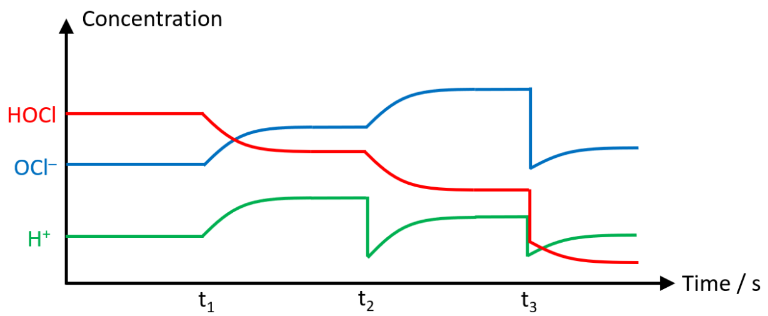
\includegraphics[width=0.80\linewidth]{assets/07_hocl_concentrations.png}
	\caption{Concentrations of \ch{H^{+}}, \ch{OCl-} and \ch{HOCl} against time}
	\label{fig:hocl}
\end{figure}

Suggest the changes necessary at \(t_1\), \(t_2\) and \(t_3\) to produce the
above graph.

\subsubsection{Solution}

We can write
\begin{equation}
	K_c = \frac{\ch{[H^{+}]} \ch{[OCl^-]}}{\ch{[HOCl]}}
	\label{eq:hocl-kc}
\end{equation}

\begin{itemize}
	\item At \(t_1\), \ch{[HOCl]} drops and \ch{[H^{+}]} and \ch{[OCl^-]} rises. \(K_c\)
	      rises. The equilibrium position is moved to the right, and {\color{accent} the
			      temperature of the solution has been increased}.
	\item At \(t_2\), \ch{[HOCl]} continues to drop gradually, \ch{[H^{+}]} drops sharply
	      and \ch{[OCl^-]} increases gradually. It is expected that both \ch{[H^{+}]} and \ch{[OCl]}
	      would continue rising under, for example, an increase in temperature, but
	      the significant drop in \ch{[H^{+}]} suggests the removal of \ch{H+} ions.
	      Therefore, {\color{accent} a strong base (e.g. \ch{NaOH (aq)}) had been added},
	      which neutralised \ch{H+} while shifting the equilibrium position to the right
	      to continue producting \ch{OCl-}.
	\item At \(t_3\), \ch{[HOCl]}, \ch{[OCl^-]} and \ch{[H^{+}]} all drop drastically. However,
	      \ch{[HOCl]} continues decreasing and \ch{[H^{+}]} and \ch{[OCl^-]} continue increasing (albeit
	      at a lower rate) after \(t_3\), suggesting that {\color{accent} the solution had been
			      diluted with \ch{H2O (l)}}.
\end{itemize}

\subsection{Trouble concentrating}
\subsubsection{Problem}

In the reaction below, \qty{4.0}{\mol} \ch{H2} and \qty{2.0}{\mol} \ch{I2} are allowed
to react in a \qty{2.0}{\dm\cubed} vessel at \qty{440}{\celsius}.
\begin{equation}
	\ch{H2 (g) + I2 (g) <=> 2 HI (g)}
\end{equation}
The equilibrium concentration of \ch{HI} is \qty{1.9}{\conc}.

Calculate the \(K_c\) for the reaction\sidenote{equilibrium constant} at
\qty{440}{\celsius}, stating its units.

\subsubsection{Solution}
\begin{align*}
	\eta_{\ch{HI}}                                                                & = \qty{1.9}{\mol\per\dm\cubed} \times \qty{2.0}{\dm\cubed}                                      \\
	                                                                              & = \qty{3.8}{\mol}                                                                               \\
	\\
	\eta_{\ch{H2}} \text{ reacted}                                                & = \slf{\qty{3.8}{\mol}}{ 2                                                                    } \\
	                                                                              & = \qty{1.9}{\mol}                                                                               \\
	\because \eta_{\ch{H2}} \text{ reacted} \colon \eta_{\ch{I2}} \text{ reacted} & = 1 \colon 1                                                                                    \\
	\eta_{\ch{H2}} \text { at eq.}                                                & = \qty{4.0}{\mol} - \qty{1.9}{\mol} = \qty{2.1}{\mol}                                           \\
	\eta_{\ch{I2}} \text { at eq.}                                                & = \qty{2.0}{\mol} - \qty{1.9}{\mol} = \qty{0.1}{\mol}                                           \\
	\\
	\ch{[H2]}                                                                     & = \slf{\qty{2.1}{\mol}}{\qty{2.0}{\dm\cubed}} = \qty{1.05}{\conc}                               \\
	\ch{[I2]}                                                                     & =  \slf{\qty{0.1}{\mol}}{\qty{2.0}{\dm\cubed}} = \qty{0.05}{\conc}                              \\
	\\
	K_c                                                                           & = \frac{\ch{[HI]}^2}{\ch{[H2]} \ch{[I2]}}                                                       \\
	                                                                              & = \frac{\ab(\qty{1.9}{\mol\per\dm\cubed})^2}{\qty{1.05}{\conc} \times \qty{0.05}{\conc}}        \\
	                                                                              & = \color{accent} \num{68.8}
\end{align*}

\subsection{Under pressure}
\subsubsection{Problem}
A sample of pure \ch{NO2 (g)} when heated to \qty{1000}{\celsius} decomposes
according to the following equation (Equation~\ref{eq:no2-decomp}):
\begin{equation}
	\ch{2 NO2 (g) <=> O2 (g) + 2 NO (g)}
	\label{eq:no2-decomp}
\end{equation}
The equilibrium constant \(K_p\) is \qty{158}{\atm}. Analysis shows that the
partial pressure of oxygen is \qty{0.25}{\atm} at equilibrium.

Calculate the partial pressures of \ch{NO} and \ch{NO2} in the equilibrium
mixture.

\subsubsection{Solution}
\begin{align*}
	K_p                              & = \frac{P_{\ch{O2}}{P_{\ch{NO}}}^2}{{P_{\ch{NO2}}}^2}             \\
	\qty{158}{\atm}                  & = \qty{0.25}{\atm} \times \ab(\frac{P_{\ch{NO}}}{P_{\ch{NO2}}})^2 \\
	\frac{P_{\ch{NO}}}{P_{\ch{NO2}}} & = \sqrt{632}
\end{align*}

Let the change in the partial pressure of \ch{NO2} be \(p\), and the initial
pressure be \(P\).

We can construct an ICE table (Table~\ref{tab:no2-decomp}).
\begin{table}[htpb]
	\centering
	\begin{tabular}{l r r r}
		\toprule
		\textbf{Pressure / \unit{\atm}} & \textbf{\ch{NO2}} & \textbf{\ch{O2}} & \textbf{\ch{NO}} \\
		\midrule
		Initial                         & \(P\)             & 0                & 0                \\
		Change                          & \(-p\)            & \(+\slf{p}{2}\)  & \(+p\)           \\
		End                             & \(P-p\)           & \(\slf{p}{2}\)   & \(p\)            \\
		\bottomrule
	\end{tabular}
	\caption{ICE table for the decomposition of \ch{NO2}}
	\label{tab:no2-decomp}
\end{table}

Given that the partial pressure of \ch{O2} is \qty{0.25}{\atm} at equilibrium,
\begin{align*}
	\slf{p}{2}                 & = \qty{0.25}{\atm}                \\
	P_{\ch{NO}} = p            & = \color{accent} \qty{0.50}{\atm} \\
	P_{\ch{NO2}} = p\sqrt{632} & = \color{accent} \qty{12.6}{\atm}
\end{align*}

\subsection{Silver salts}
\subsubsection{Problem}
Silver(I) chloride (\(K_{\text{sp}} = \num{1.82e-10}\) at \qty{298}{\kelvin}) is
a sparingly soluble salt. Silver(I) chromate(VI), \ch{Ag2CrO4}, is another
sparingly soluble salt, with \(K_{\text{sp}} = \num{1.18e-12}\) at
\qty{298}{\kelvin}.

\begin{enumerate}
	\item Calculate the solubility of silver(I) chloride in water at \qty{298}{\kelvin}.
	\item Show that \ch{Ag2CrO4} is \textbf{more} soluble in water than \ch{AgCl} at
	      \qty{298}{\kelvin} although the value of \(K_{\text{sp}}\) is smaller than
	      that of \ch{AgCl}.
\end{enumerate}

\subsubsection{Solution}
The dissolution of silver(I) chloride can be written as
\begin{equation}
	\ch{AgCl (s) <=> Ag+ (aq) + Cl- (aq)}
	\label{eq:agcl}
\end{equation}

We can thus say\sidenote{\ch{AgCl} is a solid, so there is no denominator.}

\begin{align*}
	K_{\text{sp}} & = \ch{[ Ag^{+} ]} \ch{[Cl^-]}
\end{align*}

Let the solubility of \ch{AgCl (s)} be \(S\).

\begin{align*}
	S = \ch{[AgCl]}                             & = \ch{[ Ag^{+} ]} = \ch{[Cl^-]}       \\
	K_{\text{sp}} = \ch{[ Ag^{+} ]} \ch{[Cl^-]} & = S \times S = S^2                    \\
	S                                           & = \sqrt{\num{1.82e-10}}               \\
	                                            & = \color{accent} \qty{1.35e-5}{\conc}
\end{align*}

Let the solubility of \ch{Ag2CrO4} at \qty{298}{\kelvin} be \(S_1\). We can write
\begin{equation}
	\ch{Ag2CrO4 (s) <=> 2 Ag+ (aq) + CrO4^{2-} (aq)}
	\label{eq:ag2cro4}
\end{equation}
\begin{align*}
	S_1 = \ch{[CrO4^{2-}]} & = \slf{\ch{[Ag^{+}]}}{2}           \\
	K_{\text{sp}}          & = \ch{[Ag^{+}]}^2 \ch{[CrO4^{2-}]} \\
	                       & = 4{S_1}^3                         \\
	                       & = \num{1.18e-12}                   \\
	\\
	S_1                    & = \sqrt[3]{\f{\num{1.18e-12}}{4}}  \\
	                       & = \qty{6.66e-5}{\conc}             \\
	\\
	\therefore S_1         & > S \qed
\end{align*}
{\color{accent} \ch{Ag2CrO4} is more soluble than \ch{AgCl} in water at \qty{298}{\kelvin}.}


% *** Acids and Bases ***
\chapter{Acids and Bases}
\section{Pre-lesson exercise: Acids and Bases}
\subsection{Acid--base reactions}
\subsubsection{Problem}
Which of the following are \hil{acid--base reactions}
according to the Brønsted--Lowry theory? For the acid--base
reactions in this set, identify the \hil{conjugate acid}
(with its corresponding base\sidenote{A proton-donating substance})
and the \hil[cobalt]{conjugate base} (with its corresponding acid\sidenote{A proton-accepting substance}).

\begin{itemize}
	\item \ch{H2SO4 + H2O -> HSO4- + H3O+}
	\item \ch{(CH3)3N + H2O -> (CH3)3NH^{+} + OH-}
	\item \ch{2 Na + H2O -> 2 NaOH + H2}
	\item \ch{HCl + HCO3- -> Cl- + H2CO3}
	\item \ch{Cl2 + H2 -> 2 HCl}
	\item \ch{CH4 + Cl2 -> CH3Cl + HCl}
\end{itemize}

\subsubsection{Solution}
\begin{itemize}
	\item {\color{accent} \ch{H2SO4 + H2O -> HSO4- + H3O+}}
	      \begin{itemize}
		      \item The acid is \ch{H2SO4}, and its conjugate base is \ch{HSO4-}.
		      \item The base is \ch{H2O}, and its conjugate acid is \ch{H3O+}.
	      \end{itemize}
	\item {\color{accent} \ch{(CH3)3N + H2O -> (CH3)3NH^{+} + OH-}}
	      \begin{itemize}
		      \item The acid is \ch{H2O}, and its conjugate base is \ch{OH-}.
		      \item The base is \ch{(CH3)3N}, and its conjugate acid is \ch{(CH3)3NH^{+}}.
	      \end{itemize}
	\item \ch{2 Na + H2O -> 2 NaOH + H2} is \textbf{not} an acid--base reaction.
	\item {\color{accent} \ch{HCl + HCO3- -> Cl- + H2CO3}}
	      \begin{itemize}
		      \item The acid is \ch{HCl}, and its conjugate base is \ch{Cl-}.
		      \item The base is \ch{HCO3-}, and its conjugate acid is \ch{H2CO3}.
	      \end{itemize}
	\item \ch{Cl2 + H2 -> 2 HCl} is \textbf{not} an acid--base reaction.
	\item {\color{black!40!white} \ch{CH4 + Cl2 -> CH3Cl + HCl}} is a \hil[naples]{disproportionation reaction}.
\end{itemize}

\subsection{Conjugate acids and bases}

\subsubsection{Problem}
Which of the following are
\hil[naples]{conjugate acid--base pairs}\sidenote{Two species that differ by one proton}?

\begin{enumerate}
	\item \ch{CH3CO2H} and \ch{CH3CO2-}
	\item \ch{HCO3-} and \ch{CO3^2-}
	\item \ch{SO3} and \ch{HSO3-}
	\item \ch{[Al(H2O)6]^3+} and \ch{[Al(H2O)5(OH)]^2+}
	\item \ch{BH3} and \ch{BH4-}
	\item \ch{H-} and \ch{H2}
\end{enumerate}
\subsubsection{Solution}
\begin{itemize}
	\item {\color{accent} \ch{CH3CO2H} and \ch{CH3CO2-}} are a conjugate acid--base pair.
	\item {\color{accent} \ch{HCO3-} and \ch{CO3^2-}} are a conjugate acid--base pair.
	\item \ch{SO3} and \ch{HSO3-} are \textbf{not} a conjugate acid--base pair.
	\item {\color{accent} \ch{[Al(H2O)6]^3+} and \ch{[Al(H2O)5(OH)]^2+}} are a conjugate acid--base pair.
	\item \ch{BH3} and \ch{BH4-} are \textbf{not} a conjugate acid--base pair.
	\item {\color{accent} \ch{H-} and \ch{H2}} are a conjugate acid--base pair.
\end{itemize}

% *** homework ***
\pagebreak
\section{Homework: Acids and Bases}
\subsection{Polyprotic acids}
\subsubsection{Problem}
In a \hil{polyprotic acid} \sidenote{A substance capable of donating more than one proton},
we have successive \(\Ka\) values for each successive
dissociation. For example, phosphoric acid has three dissociations, and so has
correspondingly three \(\Ka\) values, one for each dissociation (Equations~\ref{eq:polyprotic}):
\begin{align}
	% \ch{H3PO4 (aq)}     & \ch{<=>} \ch{H^{+} (aq) + H2PO4- (aq)}   \nonumber  \\
	% \ch{H2PO4- (aq)}    & \ch{<=>} \ch{H^{+} (aq) + HPO4^{2-} (aq)} \nonumber \\
	% \ch{HPO4^{2-} (aq)} & \ch{<=>} \ch{H^{+} (aq) + PO4^{3-} (aq)}
	\ch{
	H3PO4 (aq)     & <=> H^{+} (aq) + H2PO4- (aq)    \nonumber            \\
	H2PO4- (aq)    & <=> H^{+} (aq) + HPO4^{2-} (aq) \nonumber            \\
	HPO4^{2-} (aq) & <=> H^{+} (aq) + PO4^{3-} (aq) \label{eq:polyprotic}
	}
\end{align}

The corresponding \(\Ka\) values are
\begin{align*}
	K_1 & = \num{7.11e-3}  \\
	K_2 & = \num{6.32e-8}  \\
	K_3 & = \num{4.48e-13}
\end{align*}

\begin{enumerate}
	\item\label{item:decreased-ka} Suggest why, for most polyprotic acids, the successive \(\Ka\) values
	      will decrease by a large factor.
	\item\label{item:significance} \bf{Assuming only the first dissociation of phosphoric acid is significant},
	      calculate the \pH\ of \qty{0.0750}{\conc} phosphoric acid.
	\item Based on your answer to Part~\ref{item:decreased-ka}, estimate \ch{[H3PO4]},
	      \ch{[H2PO4^{-}]}, \ch{[HPO4^{2-}]} and \ch{[PO4^{3-}]} in the phosphoric acid
	      solution. From your calculations, is the assumption in Part~\ref{item:significance}
	      valid?
\end{enumerate}

\subsubsection{Solution}
It becomes more difficult for polyprotic acids to lose \ch{H+} ions with each
dissociation, since {\color{accent} \ch{H+} ions are less likely to leave an increasingly
		negatively-charged anion}.
\begin{equation*}
	K_1 = \frac{\ch{[H^{+}]} \ch{[H2PO4^{-}]}}{\ch{[H3PO4]}}
\end{equation*}
We can construct an ICE table, where \(x\) is the change in concentration of
each species (Table~\ref{tab:h3po4}).
\begin{table}[htpb]
	\centering
	\begin{tabular}{l r r r}
		\toprule
		\textbf{Concentration / \unit{\conc}} & \ch{H3PO4}           & \ch{H+} & \ch{H2PO4^{-}} \\
		\midrule
		Initial                               & \num{0.0750}         & 0       & 0              \\
		Change                                & \(-x\)               & \(+x\)  & \(+x\)         \\
		End                                   & \(\num{0.0750} - x\) & \(x\)   & \(x\)          \\
		\bottomrule
	\end{tabular}
	\caption{ICE table for the dissociation of \ch{H3PO4}}
	\label{tab:h3po4}
\end{table}

Hence, by assuming that only the dissociation of \ch{H3PO4} is significant,
\begin{align*}
	\num{7.11e-3} & = \f{x^2}{\num{0.0750} - x}  \\
	x             & = \qty{1.981e-2}{\conc}      \\
	\pH           & = -\lg x                     \\
	              & = \color{accent} \num{1.703}
\end{align*}

Hence,
\begin{align*}
	\ch{[H3PO4]}   & \approx 0.0750 - x     \\
	               & = \qty{0.05519}{\conc} \\
	\ch{[H2PO4^-]} & \approx x              \\
	               & = \qty{0.01981}{\conc}
\end{align*}

Let \(y\) be \ch{[HPO4^{2-}]} formed by the second dissociation.
\begin{align*}
	K_2 & = \f{\ch{[H^+]} \ch{[HPO4^{2-}]}}{\ch{[H2PO4^-]} - y} \\
	    & = \f{y \ab(y + \num{0.01981})}{\num{0.01981} - y}     \\
	y   & = \qty{6.3e-8}{\conc}
\end{align*}

Since \(y\) is minuscule compared to \(x\), the assumption in
Part~\ref{item:significance} can be accepted.

Let \(z\) be \ch{[PO4^{3-}]} formed by the third dissociation.
\begin{align*}
	K_3 & = \f{\ch{[H^+]} \ch{[PO4^{3-}]}}{\ch{[H2PO4^-]} - z} \\
	    & = \f{z \ab(z + \num{0.01981})}{y-z}                  \\
	z   & \approx 0
\end{align*}
Since \(z \approx 0\), the assumption in
Part~\ref{item:significance} can be accepted for the third dissociation also.

\subsection{Titration curves}
\subsubsection{Problem}
Sketch the titration curve of \ch{H2SO3}, a diprotic weak acid, against
\ch{NaOH} \sidenote{\ch{NaOH} is a strong base.}.
Suggest the indicators you would add in order to see both end points clearly, and
state their colour changes.

\subsubsection{Solution}
\ch{H2SO3} dissociates according to the following equations:
\begin{align*}
	\ch{H2SO3 (aq)  & <=> HSO3^- (aq) + H^+ (aq)}   \\
	\ch{HSO3^- (aq) & <=> SO3^{2-} (aq) + H^+ (aq)}
\end{align*}
Since \ch{H2SO3} is a weak acid, the increase in \pH\ will be more gradual
than those expected with a strong acid.
\begin{figure}[htpb]
	\centering
	\begin{tikzpicture}
		\begin{axis}[ticks=none, xlabel={Volume of \ch{NaOH} added}, ylabel={pH}]
			% Adding points manually based on assumed calculations
			\addplot[
				smooth,
			] coordinates {
					% step 1
					(0, 1.9) (5, 1.93) (10, 1.95) (15, 1.975)
					(20, 2) (22, 2.1) (24, 2.25) (26, 2.35)
					(28, 2.4) (30, 2.5) (32, 2.7) (34, 2.9)
					(36, 3.2) (38, 3.5) (39, 3.75) (40, 4)
					% step 2
					(42, 4.5) (44, 5) (46, 5.5) (48, 6) (50, 6.2)
					(52, 6.4) (54, 6.6) (56, 6.8) (58, 6.9) (59, 6.95)
					(60, 7) (61, 7.05) (62, 7.07) (63, 7.1) (65, 7.15)
					(67, 7.2) (68, 7.22) (70, 7.24) (72, 7.51) (74, 7.82)
					(76, 8.44) (78, 8.87) (79, 9.5) (80, 10) (82.5, 10.5)
					(85, 11) (87.5, 11.5) (89, 12) (90, 12) (95, 12) (97, 12)
					(100, 12) (105, 12) (110, 12) (115, 12) (118, 12) (120, 12)
				};
			\addplot+ [only marks] coordinates {
					(40, 4) (80, 10)
				};
		\end{axis}
	\end{tikzpicture}
	\caption{Titration curve of \ch{H2SO3} with \ch{NaOH}}
	\label{fig:titration-h2so3}
\end{figure}

The titration curve is in Figure~\ref{fig:titration-h2so3}. We can use {\color{accent}
		methyl orange} for the first endpoint, and {\color{accent} phenolphthalein} for the second.

\subsection{Liquid--liquid extraction}
\subsubsection{Problem}
Liquid--liquid extraction (Figure~\ref{fig:ll-sep}) is a technique to separate
organic compounds using a separatory funnel. The crude sample is first dissolved
in an organic solvent such as hexane and this solution is poured into a separatory funnel.
Next, water is added to the separatory funnel and the funnel is shaken.
Because hexane and water are immiscible, they form two layers in the
separatory funnel. The organic compound that is more soluble in water will migrate
from the hexane layer to the water layer. The two layers contain different
compounds and can be collected separately.

\begin{wrapfigure}{r}{0.5\textwidth}
	\centering
	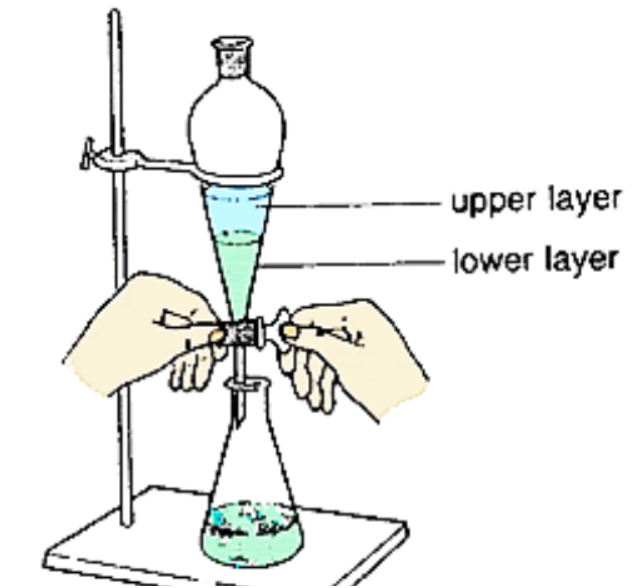
\includegraphics[width=0.5\linewidth]{assets/08_ll_separation.png}
	\caption{Liquid--liquid separation}
	\label{fig:ll-sep}
\end{wrapfigure}

You are given a sample containing both phenol (\(\pKa = \num{9.95}\)) and benzoic
acid (\(\pKa = \num{4.20}\)). Both compounds are not very soluble in water. To
improve the separation, aqueous sodium bicarbonate (\ch{NaHCO3}) can be used instead
of water.

It is given that \(\pKa_1 = \num{6.3}\) and \(\pKa_2 = \num{10.3}\) for carbonic
acid, \ch{H2CO3}. In which layer will the majority of the benzoic acid be found?
In which layer will the majority of the phenol be found? You need not perform
equilibrium computations.

\subsubsection{Solution}
\ch{NaHCO3} is a weak base. We can write
\begin{equation*}
	\ch{HCO3^- (aq) <=> CO3^{2-} (aq) + H^+ (aq)}
\end{equation*}
We can also write the dissociation of \ch{H2CO3 (aq)} as
\begin{align*}
	\ch{H2CO3 (aq)    & <=> HCO3^{-} (aq) + H^+ (aq)} \\
	\ch{HCO3^{-} (aq) & <=> CO3^{2-} (aq) + H^+ (aq)}
\end{align*}
It is the \it{second} dissociation of \ch{H2CO3 (aq)} we desire. We use
\(\pKa \coloneqq \pKa_2 = \num{10.3}\).

Since the \pKa\ of benzoic acid (\num{4.20}) is smaller than that of phenol
(\num{9.95}), it has a larger \Ka\ and hence is the stronger acid. It will react
more readily with the \ch{NaHCO3 (aq)} to form benzoate ions, which are soluble
in water. {\color{accent} The majority of the benzoic acid will be found in the
		aqueous layer.}

On the other hand, the \pKa\ values of phenol and \ch{H2CO3 (aq)} are closer
to each other, making the acid--base reaction less favourable. {\color{accent}
		Phenol will predominantly be found in the hexane layer.}


% Electrochemistry
\chapter{Electrochemistry}
\section{Pre-lesson exercise: Electrochemistry}
\subsection{Metals}
\subsubsection{Problem}
\bf{W}, \bf{X}, \bf{Y} and \bf{Z} are four unknown metals.

\bf{Y} does not react with water.

Precipitation is observed when solid \bf{W} is added into a solution of \bf{Z}
chloride.  No visible change is observed when solid \bf{W} is added into a solution
of \bf{Y} chloride.

Based on the above information, match the following metals to the correct
letters:
\begin{itemize}
	\item \ch{Mg}
	\item \ch{Al}
	\item \ch{Fe}
	\item \ch{Cu}
\end{itemize}

\subsubsection{Solution}

Since \bf{W} displaces \bf{Z} but not \bf{Y}, \bf{W} is more reactive than \bf{Z}
but less reactive than \bf{Y}. However, \bf{Y} does not react with water,
indicating that it is not highly reactive.

We can conclude that:
\begin{itemize}
	\item {\color{accent} \bf{W} is iron}. It has a reactivity in between that of two metals.
	\item {\color{accent} \bf{Z} is copper}. It has the lowest reactivity, since \bf{W} could displace it.
	\item {\color{accent} \bf{Y} is aluminium}. It is more reactive than \bf{W}, yet cannot dissolve in water, indicating that its reactivity is not the highest.
	\item {\color{accent} \bf{X} is, therefore, magnesium}.
\end{itemize}

\subsection{Electrolysis}
\subsubsection{Problem}
The electrolysis of dilute sodium nitrate was conducted as shown in Figure~\ref{fig:electrolysis-nano3}.
\begin{figure}[htpb]
	\centering
	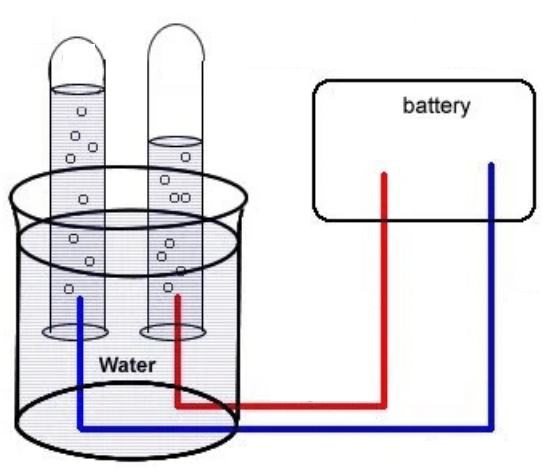
\includegraphics[width=0.4\linewidth]{assets/09_electrolysis_nano3.png}
	\caption{Electrolysis of \ch{NaNO3 (aq)}}
	\label{fig:electrolysis-nano3}
\end{figure}
\begin{enumerate}
	\item\label{part:no3-discharge} With reference to oxidation numbers, explain why the nitrate anion will not be discharged.
	\item\label{part:na-discharge} Explain why the sodium cation will not be discharged.
	\item Despite Parts~\ref{part:no3-discharge} and~\ref{part:na-discharge}, explain why
	      the electrolysis will not work without sodium nitrate.
	\item By considering the oxidation and reduction reactions taking place, label the following on the diagram:
	      \begin{itemize}
		      \item the polarity of the battery (\(+\) or \(-\)),
		      \item the anode and the cathode, and
		      \item the flow of electrons, and the flow of electrical current.
	      \end{itemize}
	\item State what will be observed when a few drops of universal \pH\ indicator
	      are added into the solution.
\end{enumerate}

\subsubsection{Solution}
\ch{N} in \ch{NO3^-} has an oxidation state of \(+5\). Since \ch{N} is in
group 15 in the periodic table, \(+5\) is its maximum oxidation state. Since \ch{NO3^-}
is an anion, one would expect it to be oxidised at the anode. However, the
oxidation of \ch{NO3^-} is defined as the increase in oxidation state of \ch{N},
which is impossible. Therefore, \ch{NO3^-} cannot be oxidised.

The competing species at the cathode (to be reduced) are \ch{Na^+} and \ch{H2O}, since the electrolyte
is an aqueous solution. \ch{H2O}, however, is lower in the electrochemical series,
so it is preferentially reduced over \ch{Na^+}. The reduction of \ch{H2O}
forms \ch{H2 (g)}, and the reduction of \ch{Na^+} will only take place once
all \ch{H2O} has been reduced/oxidised.

Without \ch{NaNO3 (aq)}, only \ch{H2O (l)} would be present in the electrolyte.
Assuming that \ch{H2O (l)} is deionised for the purposes of this electrolysis, it
will not allow electron flow without mobile ions which act as mobile charge carriers.

The annotated diagram is in Figure~\ref{fig:nano3-ans}.

\begin{figure}[htpb]
	\centering
	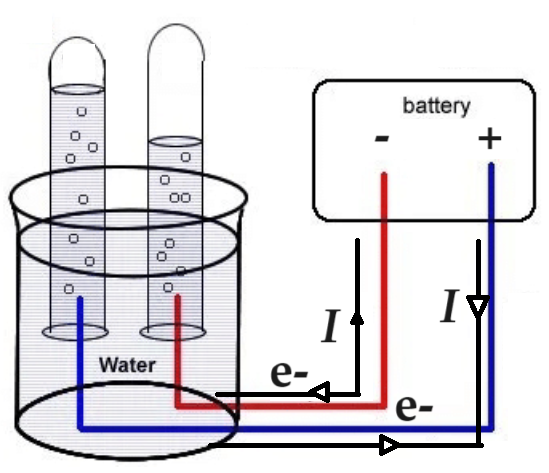
\includegraphics[width=0.4\linewidth]{assets/09_electrolysis_nano3_ans.png}
	\caption{Annotated electrolysis diagram}
	\label{fig:nano3-ans}
\end{figure}

\ch{H2O (l)} is both preferentially reduced and oxidised at the cathode and anode
respectively.
\begin{align*}
	\ch{2 H2O (l) + 2 e^- & <=> H2 (g) + 2 OH^- (aq)}            \\
	\ch{H2O (l)           & <=> 1/2 O2 (g) + 2 H^+ (aq) + 2 e^-}
\end{align*}
For the same number of moles of electrons passed through the electrolyte, the
number of moles of \ch{OH^-} and \ch{H^+} produced are equal. The overall \pH\
of the solution does not change.

However, \ch{H^+} ions are produced at the anode, meaning that the solution surrounding
the anode will turn {\color{accent} acidic}. {\color{accent} Near the anode, the green universal
\pH\ indicator will turn red}.

\ch{OH^-} ions are produced at the cathode, meaning that the solution surrounding
the cathode will turn {\color{cobalt} basic}. {\color{cobalt} Near the cathode, the green universal \pH\ indicator will turn purple.}

\end{document}